
\chapter{Software Version Control}
Die wichtigsten Aufgaben eines Versionsverwaltungssystems
sind:
\begin{enumerate}
\item
% die Speicherung der Fileversionen (Revisions) mit \"Anderungskommentar,
 die Protokollierung der Änderungen, damit jederzeit nachvollzogen
                 werden kann, wer wann was (warum) geändert hat.
\item die eindeutige Kennzeichnung der Versionen und ihrer
  Abhängigkeiten (Baumstruktur),
\item die Zugriffsregelung und (wenn möglich) automatische Abgleichung
  bei gleichzeitigen Modifikationen (Mehrbenutzerfähigkeit),
\item Wiederherstellung bestimmter Änderungszustände/Releases
% die Gruppierung von Fileversionen zu Releases (Snapshots)
%\item
% Gleichzeitige Entwicklung mehrerer Entwicklungszweige (engl. Branches) eines
% Projektes (z.B. stabile Release-Version und  und Entwicklerversion mit
% größeren, nicht getesteten Änderungen)
\end{enumerate}
\ifslides
\newpage
\fi
Es existieren zahlreiche kommerzielle und freie Softwarepakete, die sich in
die beiden Kategorien einteilen lassen:
\begin{description}
\item[Zentrale Systeme] Diese Systeme zeichnen sich durch eine zentrales
  Archiv (Repository) aus, wo die Originaldateien abgelegt sind. Beispiele sind:
  \begin{itemize}
  \item CVS: früher weit verbreitet
  \item Subversion: Nachfolger von CVS mit einigen Verbesserungen
  \end{itemize}
\item[Dezentrale Systeme] bei diesen Systemen sind die Dateien lokal auf den
  jeweiligen Entwicklungssystemen abgelegt (Distributed Version
  Control System DVCS). Beispiele sind:
  \begin{itemize}
  \item GNU Arch
  \item Bazaar-NG
  \item BitKeeper (kommerziell)
  \item Git
  \item Monotone
  \item Mercurial
  \end{itemize}
\end{description}
\ifslides
\newpage
\fi
Ein weiteres Unterscheidungsmerkmal ist die Arbeitsweise:
\begin{description}
\item[Lock-Modify-Unlock] (Pessimistic Revision Control) Einzelne Dateien müssen vor einer
  Än\-derung gesperrt und nach Abschluss der Änderung wieder freigegeben werden.
\item[Copy-Modify-Merge] (Optimistic Revision Control)
   Die Dateien können von allen Benutzern
  geändert werden. Gleichzeitig durchgeführte Änderungen werden anschliessend
  entweder automatisch oder manuell zusammengeführt.
\end{description}
%%% End:
\newslide
\newpage
\section{Git}
GIT\footnote{englischer Slangausdruck: Blödmann, Depp}
 ist ein einfaches, von Linus Torvalds 2005 für das
 Linux-Kernel-Projekt
in wenigen Monaten entwickeltes
Versionsverwaltungssystem. Torvalds nennt es ein ``stupid
(but extremely fast) directory content manager''. Anstoss dazu gab eine
längere Auseinandersetzung mit dem Hersteller von BitKeeper, dem bis anhin von
den Kernel-Entwicklern eingesetzten
Versionsverwaltungssystems. Hauptkritikpunkt
an CVS und anderen quell-offenen Paketen waren Performance-Probleme, die bei
der grossen Anzahl von Dateien (mehr als 30 000) und der hohen Änderungsrate
auftraten: ``Taking tens of seconds to apply a patch just because the source
base is big is just not acceptable''. Mittlerweile geniesst Git (nebst
Mercurial) eine grosse Popularität und wird in einer wachsenden Zahl von
kleinen bis hin zu sehr grossen Projekten eingesetzt.

\newslide
Wichtige Unterschiede zu Subversion sind
\begin{itemize}
\item \structure{Verteilte Repositories}: jede/r
Bearbeiter/-in hat ein eigenes, lokales Repository im Unterverzeichnis
.git des Arbeitsverzeichnis. Ein spezielles Repository,
ein sogenanntes ``Bare Repository'', kann eingerichtet werden
um die Dateien anderen zugänglich zu machen.
\item \structure{Branches und Tags}: es gibt keine
  Trunk/Tags/Branches-Verzeichnisse. Tags und Branches sind Teil
  des Repository's.
\item \structure{Revision-Bezeichner}: Statt ganzzahliger
  Revision-Bezeichner werden SHA1-Werte verwendet.
  Die aktuellste Revision kann mit dem Bezeichner HEAD referenziert werden.
\item \structure{Snapshots statt Änderungen}:
     Git speichert keine Änderungen, sondern bildet bei
jedem Commit einen Snapshot, der ein komprimiertes Abbild aller
verwalteten Dateien darstellt. (Unveränderte Dateien werden verlinkt).
\item \structure{Zustände}: Dateien haben einen Zustand: untracked,
  modified, staged, commited
\end{itemize}

%\begin{itemize}
%
% http://wiki.phys.ethz.ch/readme/git_basics
%\item Single Repository Coupled with the Project
%\item Synchronizing Production and Developer Copies
%\item Bare repository
%\end{itemize}

%
%Eigenschaften;
%\begin{itemize}
%\item Git ist eher ein Dateisystem als eine klassische Versionsverwaltung.
%\item Fast alle Operationen sind lokal
%\end{itemize}

Git unterscheidet 4 Objekt-Typen:
\begin{itemize}
\item \structure{Blob}: eine Byte-Sequenz (eine Datei: Text, Bild etc.)
\item \structure{Tree}: ein Verzeichnis, kann Blobs und andere Trees enthalten
\item \structure{Commit}: ein Zustand, enthält einen Verweis auf den Tree, einen
  Parent und Meta-Informationen (Autor, Zeitstempel etc.)
\item \structure{Tag}: eine Markierung eines Commits
\end{itemize}
%\ifslides
%\else
%\newpage
%\fi
Alle Git-Objekte besitzen einen 160bit-Hash-Key, der
 mit 40 ASCII-Zeichen (Hex-Code)
dargestellt wird:
\begin{lstlisting}
6ff87c4664981e4397625791c8ea3bbb5f2279a3
\end{lstlisting}
Git-Objekte sind dadurch mit sehr hoher Wahrscheinlichkeit global
eindeutig.

\newslide
Git-Objekte sind im Verzeichnis .git/objects abgelegt und bilden einen
Directed Acyclic Graph (DAG):
\ifslides
\begin{center}
  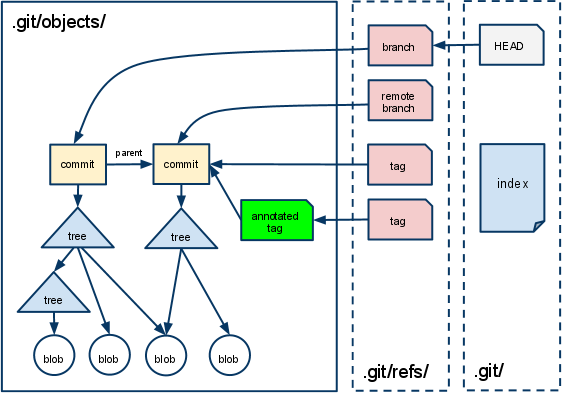
\includegraphics[width=0.7\linewidth]{config-management/git-objects}
\end{center}
\else
\begin{figure}[H]
  \centering
  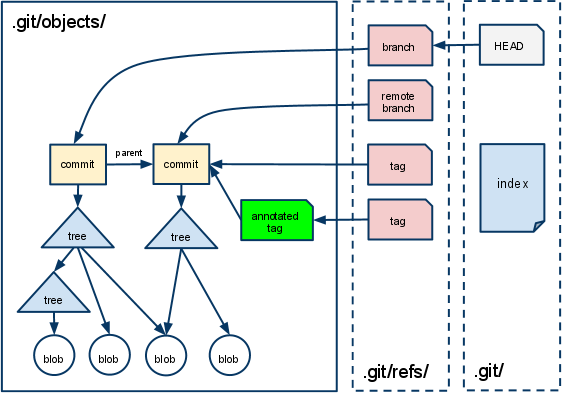
\includegraphics[width=0.7\linewidth]{config-management/git-objects}
  \caption[Git-Objekte und Referenzen]{Git-Objekte und Referenzen \\
(Source: \href{http://teohm.github.com/blog/2011/05/30/learning-git-internals-by-example}
                {teohm.github.com/blog/2011/05/30/learning-git-internals-by-example})}
  \label{fig:gitobjects}
\end{figure}
\fi
\newslide
Ein Hauptvorteil von Git gegenüber anderen Systemen ist der sehr
flexible und einfache Umgang mit Branches, die bei
Git eine wichtige Rolle spielen. Branches werden
zum Beispiel verwendet für
\begin{itemize}
\item das Durchführen von Experimenten
\item das Ausprobieren von Ideen
\item die Entwicklung verschiedener Features
\end{itemize}
oder ganz allgemein, wenn man etwas modifzieren möchte.

Git ist mehr als nur ein Werkzeug, es ist auch ein Paradigma.
Es bringt neue Ideen und
räumt mit einigen bisher als inhärent geltenden Einschränkungen auf.
Wenn man git verwendet, vergisst man am besten, was man bisher über
Versionsverwaltung zu wissen glaubte.
%
\newslide
\subsection{Die wichtigsten Befehle}
\ifslides
\begin{center}
  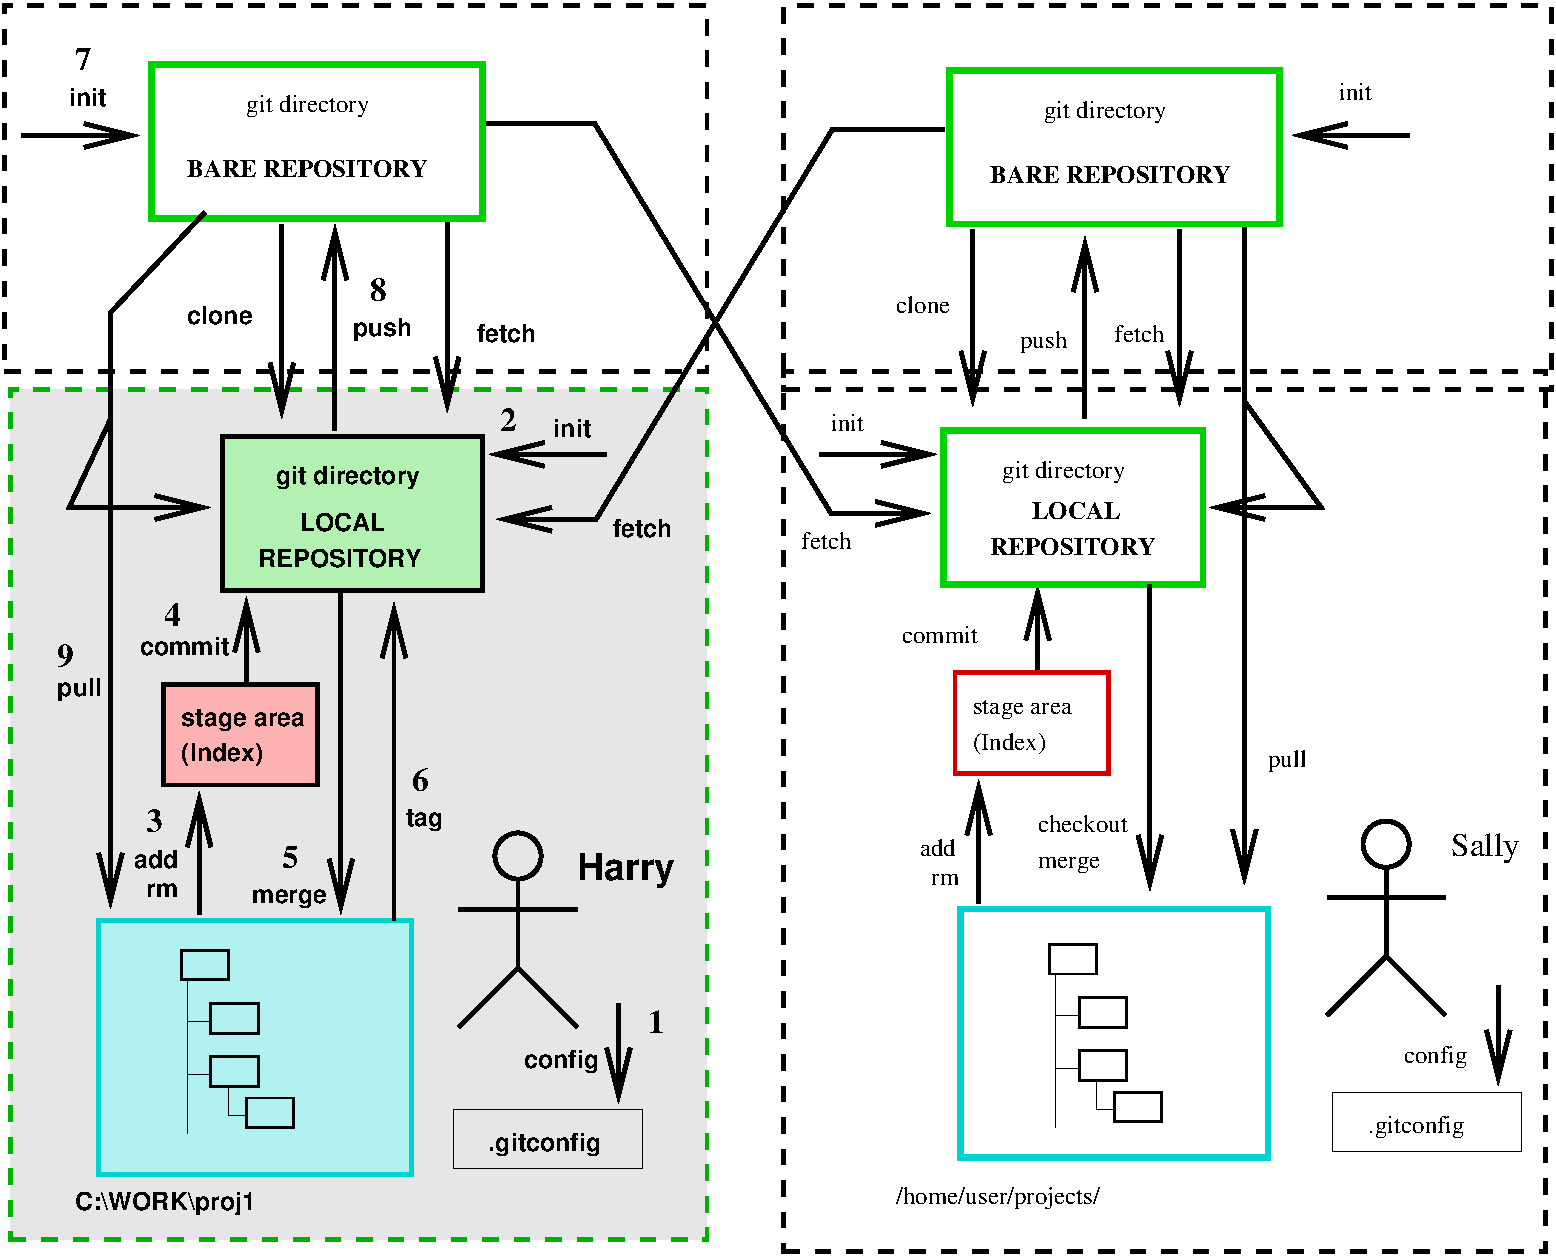
\includegraphics[width=0.65\linewidth]{config-management/xfig/git-workflow}
\end{center}
\else
\begin{figure}[H]
\centering
  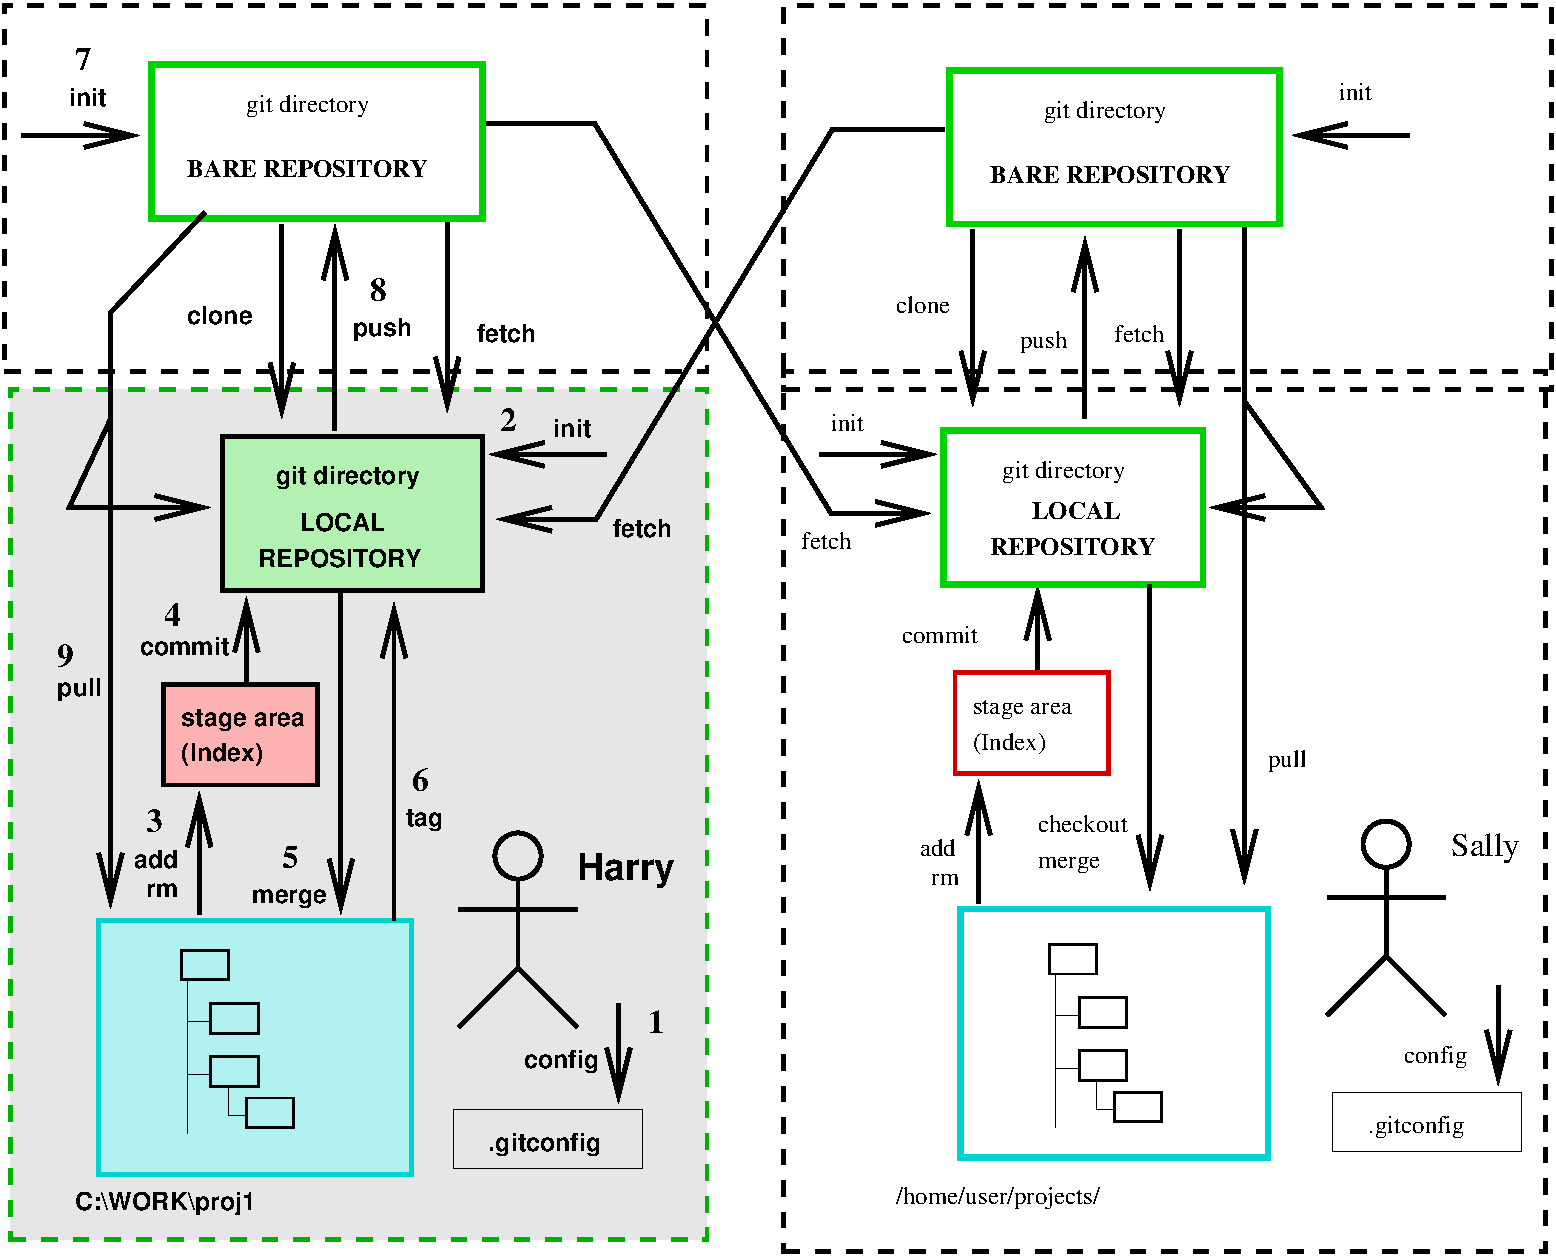
\includegraphics[width=0.95\linewidth]{config-management/xfig/git-workflow}
\caption{Der typische Arbeitsablauf bei Git}
\end{figure}
\fi
\begin{enumerate}
\item \underline{config}: Benutzername und E-Mail-Adresse festlegen:
  \begin{lstlisting}
$ git config --global user.name "Ronald Tanner"
$ git config --global user.email "ronald.u.tanner@gmail.com"
  \end{lstlisting}
Dadurch wird im Home-Verzeichnis die Datei \verb+.gitconfig+ angelegt.

Es gibt 3 Orte für
Config-Dateien: per User, per Repository, per System. Lässt man
die
Option \verb+--global+ weg, dann wird die Einstellung in der
Config-Datei des aktuellen Repository's abgelegt.
%
\newslide
\item \underline{init}: ein neues Repository einrichten. Man
  unterscheidet lokale (private) und synchronisierbare (shared)
  Repositories, die anderen Benutzer zugänglich gemacht werden können.

Ein leeres, lokales Repository im aktuellen Verzeichnis einrichten:
  \begin{lstlisting}
$ cd /home/user/projects
$ git init project1
Initialized empty Git repository in /home/user/projects/project1/.git
  \end{lstlisting}
\begin{center}
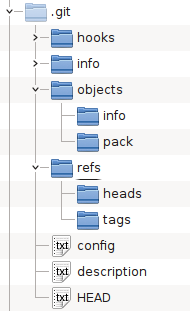
\includegraphics[width=0.25\linewidth]{config-management/git-repository-files}
\end{center}
%
{\bfseries Bemerkung:} Um ein lokales Repository aus einem bereits existierenden
zu erzeugen, muss anstelle von ``init'' der Befehl ``clone'' verwendet
werden:
\begin{lstlisting}
$ git clone file:///var/git/project1.git
\end{lstlisting}
%
\newslide
\item \underline{add}: Dateien in den Index aufnehmen.
  \begin{lstlisting}
$ cd project1
$ git add .
  \end{lstlisting}
%$
Alle im aktuellen Verzeichnis liegenden Dateien und Unterverzeichnisse
werden in die Versionsverwaltung aufgenommen (genauer: dem
Stage-Bereich, resp. dem Index hinzugefügt)
%%% git config --global http:sslVerify false
%% env GIT_SSL_NO_VERIFY=true git clone ....
%
\newslide
\begin{center}
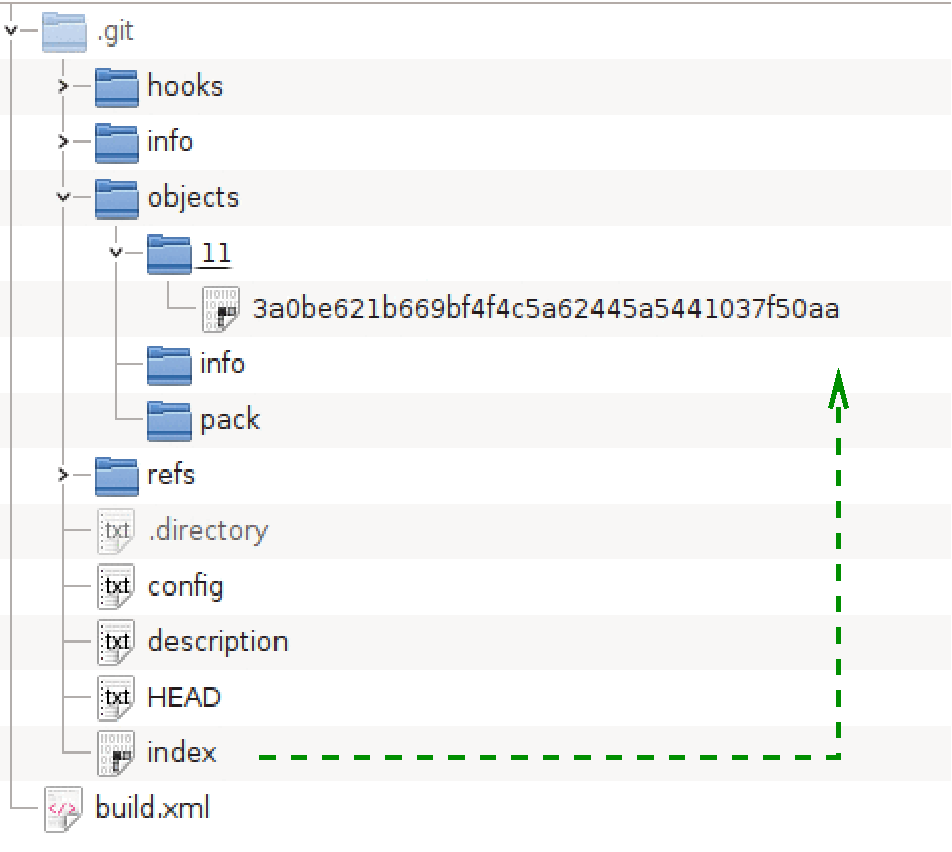
\includegraphics[width=0.7\linewidth]{config-management/xfig/git-added}
\end{center}
%% show index
%% git ls-files --stage
%%
%%%Inhalt anzeigen: git show d2ad210a...
%% 1. cat .git/HEAD:
%%    refs/heads/master
%% 2. cat .git/refs/heads/master
%%    f0dda106c105f9b15b379678d8d88322da5abd2d
%% 3. git cat-file -p f0dda106c105f9b15b379678d8d88322da5abd2d
%%    tree e4978d4515571fce768e1bb11b492e42faae7389
%%    author Ronald Tanner <tar@semafor.ch> 1410001976 +0200
%%    committer Ronald Tanner <tar@semafor.ch> 1410001976 +0200
%%
%%    initial commit
%% 4. git cat-file -p e4978d4515571fce768e1bb11b492e42faae7389
%%    100644 blob 113a0be621b669bf4f4c5a62445a5441037f50aa    build.xml
%%
%% ----------------
%% keep password
%% git config --global credential.helper cache
%%
\newslide
\item \underline{commit}: übertragen der Änderungen aus dem Index in
  den Master-Branch des Repository's:
  \begin{lstlisting}
$ git commit -m "initial commit"
  \end{lstlisting}
%$
{\bfseries Bemerkung}: modifizierte Dateien müssen vorgängig mit ``add'' in den
  Stage-Bereich kopiert werden, wenn sie in das Repository übertragen
  werden sollen. Will man alle modifizierten Dateien übertragen, kann
  man auch die Option ``-a'' angeben:
  \begin{lstlisting}
$ git commit -am "another commit"
  \end{lstlisting}
%%% $
\begin{center}
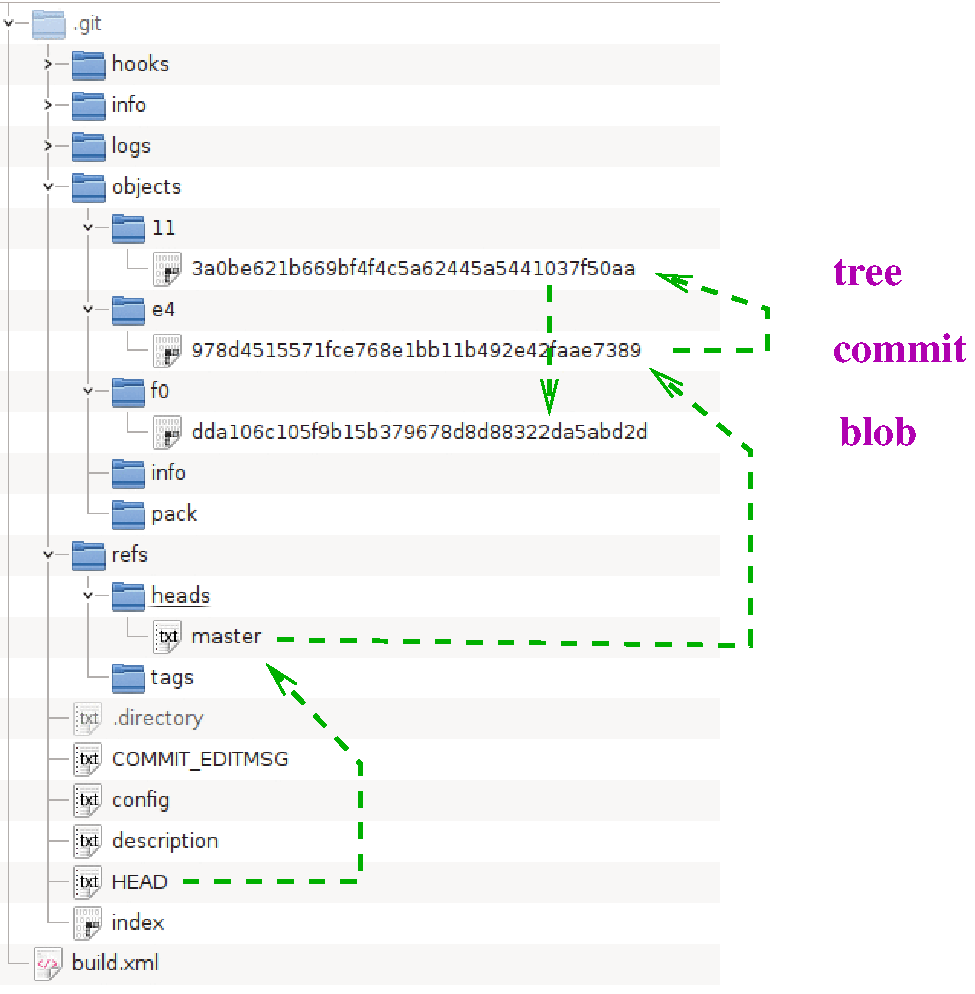
\includegraphics[width=0.66\linewidth]{config-management/xfig/git-commited}
\end{center}
\newslide
\item \underline{checkout}: das aktuelle Verzeichnis mit dem
  Inhalt des lokalen Repository's aktualisieren.
Üblicherweise wird dazu ein neuer Branch erstellt:
  \begin{lstlisting}
$ git checkout -b ticket-53
  \end{lstlisting}
%$
\newslide
\item \underline{tag}: Markierungen erzeugen, anzeigen, löschen und
  verifizieren. Eine neue Markierung des letzten Commit-Objektes erstellen:
\begin{lstlisting}
$ git tag -a rel-0.0 -m "Release 0.0"
\end{lstlisting}
%$
{\bfseries Bemerkungen}: Man unterscheidet lighweight und annotated
Tags. Lightweight Tags werden ohne die Option \verb+-a+ (und ohne
Kommentar) erstellt. Sie sind lediglich eine Referenz zu einem
speziellen Commit. Annoted Tags werden als Objekte im Repository
gespeichert und sind die bevorzugte Variante.

Alle Markierungen anzeigen:
\begin{lstlisting}
$ git tag -l
\end{lstlisting}
%$
\newslide
\item \underline{init}:
Ein leeres, synchronisierbares Repository einrichten:
\begin{lstlisting}
$ git init --bare /var/git/project1.git
\end{lstlisting}
%$
{\bfseries Bemerkung}: Bei Verwendung des Git-Daemons sollte das Repository
 dem Benutzer nobody gehören
und der Benutzergruppe gitusers Lese- und Schreibberechtigung
zugewiesen werden.
Dazu muss jedoch der entsprechende Mount-Eintrag in /etc/fstab mit der
Option acl (Access Control List) ergänzt werden. Beispiel:
\begin{verbatim}
/dev/sda3  /	ext3	noatime,acl	0 1
\end{verbatim}
Die Anweisungen lauten in diesem Fall:
\begin{lstlisting}
$ sudo groupadd gitusers
$ sudo mkdir /var/git
$ sudo chown nobody:nobody /var/git
$ sudo -u nobody git init --bare /var/git/project1.git
$ sudo setfacl -R -d -m g:gitusers:rwX /var/git/project1.git
\end{lstlisting}
% Siehe
% http://www.techrepublic.com/article/learn-to-use-extended-filesystem-acls/6091748
%  mount -v -o remount /
%$ sudo usermod -a -G gitusers tar
%
\newslide
\item \underline{push}: übertragen des Master-Branches
 des lokalen Repository's in ein
  (oder mehrere) Remote-Repository:
  \begin{lstlisting}
$ git remote add origin file:///var/git/project1
$ git push origin master
  \end{lstlisting}
{\bfseries Bemerkungen}:
\begin{itemize}
\item der Benutzer benötigt Schreibberechtigung
im Remote-Repository.
\item Mit ``remote add'' wird ein Alias für ein Remote-Repository
  definiert (Hier: origin)
\item Anzeige aller Remote-Repositories mit URL:
  \begin{lstlisting}
$ git remote -v
  \end{lstlisting}
%$
\item Tags werden nicht automatisch aus dem lokalen Repository
  übertragen. Sie müssen explizit angegeben werden:
  \begin{lstlisting}
$ git push origin rel-0.0
  \end{lstlisting}
%$
oder alle zusammen:
\begin{lstlisting}
$ git push origin --tags
\end{lstlisting}
\end{itemize}
%
\item \underline{pull}: übertragen der Daten aus dem (default)
  Remote-Repository's in das lokale Repository (fetch) und
  zusammenfügen der Änderungen mit dem aktuellen Branch (merge)
  \begin{lstlisting}
$ git pull
\end{lstlisting}
\end{enumerate}
%$
{\bfseries Bemerkung}: in der Git-Config-Datei sollte/kann das Default-Repository
und der Default-Branch definiert werden:
  \begin{lstlisting}
git config branch.master.remote origin
git config branch.master.merge refs/heads/master
  \end{lstlisting}
Nach einer Git-Clone-Operation sind diese Werte automatisch gesetzt.
%
\subsection{Weitere Funktionen}
\begin{itemize}
\item Eine bestimmte Version wiederherstellen (mit Release-Nummer):
  \begin{lstlisting}
$ git checkout -b branch-0 rel-0.0
  \end{lstlisting}
%$
\item Anzeige der Änderungen einer Datei:
\begin{lstlisting}
$ git log Main.java
\end{lstlisting}
%$
\item Detaillierte Anzeige der letzten beiden Änderungen einer Datei:
\begin{lstlisting}
$ git log -p -2 Main.java
\end{lstlisting}
%$
\item Detaillierte Anzeige Änderungen der letzten beiden Wochen:
\begin{lstlisting}
$ git log --sinde=2.weeks
\end{lstlisting}
%$
\item Vergleich der Änderungen einer Datei mit Stage-Bereich:
\begin{lstlisting}
$ git diff Main.java
\end{lstlisting}
%$
\item Vergleich zwischen Stage-Bereich und Repository:
\begin{lstlisting}
$ git diff --staged
\end{lstlisting}
%$
\item Dateien entfernen:
\begin{lstlisting}
$ git rm Main.java
\end{lstlisting}
Die Datei wird nach einem Commit im Repository als gelöscht markiert.
% $
\item eine Datei umbenennen (verschieben):
\begin{lstlisting}
$ git mv Main.java NewMain.java
\end{lstlisting}
Die Änderung wird nach einem Commit in das Repository übertragen.
%$
\item Zustand der Dateien im aktuellen Verzeichnis und darunter anzeigen
\begin{lstlisting}
$ git status
\end{lstlisting}
\end{itemize}
%$
\subsection{Verzweigungen (Branches)}
Änderungen werden bei Git in der Regel nicht direkt auf dem
Master-Branch sondern in einem separaten Branch durchgeführt, der
(in der Regel)
nach Abschluss der Änderungen mit dem Master-Branch zusammengeführt und
anschliessend gelöscht wird:
\begin{itemize}
\item Einen neuen Branch erstellen:
\begin{lstlisting}
$ git checkout -b ticket-53
\end{lstlisting}
%$
\item Alle Branches anzeigen:
  \begin{lstlisting}
$ git branch
  \end{lstlisting}
{\bfseries Bemerkung}: mit -a werden auch die Remote-Branches angezeigt
%$
\item Rückgabe der Änderungen:
  \begin{lstlisting}
$ git commit -m "initial commit"
  \end{lstlisting}
%$
\item Zum Master-Branch wechseln und zusammenführen
  \begin{lstlisting}
$ git checkout master
$ git merge ticket-53
  \end{lstlisting}
Wenn dabei keine Konflikte auftreten, werden die Änderungen
automatisch in das Repository übertragen.
\item Löschen des Branches
  \begin{lstlisting}
$ git branch -d ticket-53
  \end{lstlisting}
%$
\end{itemize}
%
\newslide
\subsection{Konfliktbehandlung}
Wenn 2 oder mehr Entwickler ihre Änderungen in ein gemeinsames
Remote-Repository übertragen, oder 2 oder mehr Branches zusammengefügt
werden, kann es zu Konflikten kommen.

Beispiel:
\begin{lstlisting}[escapechar=\%]
$ %{\bfseries git push origin master}%
To file:///var/git/project1.git
 ! [rejected]        master -> master (non-fast-forward)
error: failed to push some refs to 'file:///var/git/project1.git'
To prevent you from losing history, non-fast-forward updates were rejected
Merge the remote changes (e.g. 'git pull') before pushing again.  See the
'Note about fast-forwards' section of 'git push --help' for details.
\end{lstlisting}
%$
\newslide
Nach einem Git-Pull können folgende Meldungen angezeigt werden:
\begin{lstlisting}
Auto-merging <filename>
CONFLICT (content): Merge conflict in <filename>
Automatic merge failed; fix conflicts and then commit the result
\end{lstlisting}
Die Konfliktstellen der betreffenden Dateien sind
ähnlich wie bei Subversion markiert mit den Zeilen
\begin{lstlisting}
<<<<<<<
=======
>>>>>>>
\end{lstlisting}
Diese Stellen müssen korrigiert werden, bevor man die Änderungen per
commit übertragen kann.
% Bei
% der Bezeichnung project1.git handelt es sich eine Namenskonvention.
%
% http://www.thomas-krenn.com/de/wiki/Git_Workflows
\newslide
\subsection{Verteilte Repositories: Workflow}
Source: \href{http://git-scm.com/book/en/Distributed-Git-Distributed-Workflows}
  {Distributed-Git-Distributed-Workflows}
\begin{itemize}
\item Zentralisierter Workflow:
\begin{center}
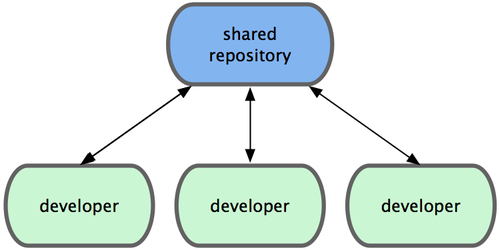
\includegraphics[width=0.6\linewidth]{config-management/git-centralized-wf}
\end{center}
\newslide
\item Integration-Manager-Workflow:
\begin{center}
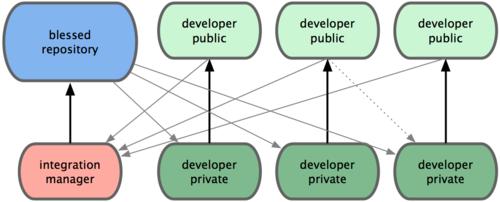
\includegraphics[width=0.75\linewidth]{config-management/git-integration-wf}
\end{center}
\newslide
\item Diktator und Leutnant:
\begin{center}
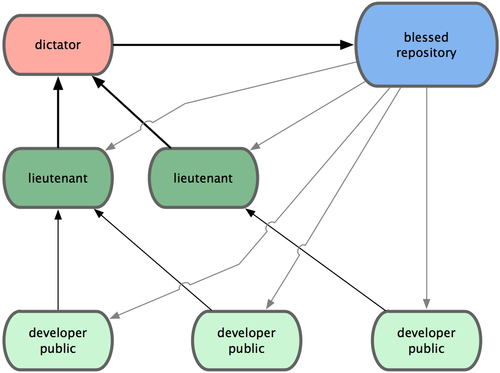
\includegraphics[width=0.75\linewidth]{config-management/git-dictator-wf}
\end{center}
\end{itemize}
% http://git-scm.com/book/en/Distributed-Git-Distributed-Workflows
\newslide
\subsection{Gitflow Workflow (Vincent Driessen)}
Source: \href{http://nvie.com/posts/a-successful-git-branching-model}
  {nvie.com/posts/a-successful-git-branching-model}
\begin{center}
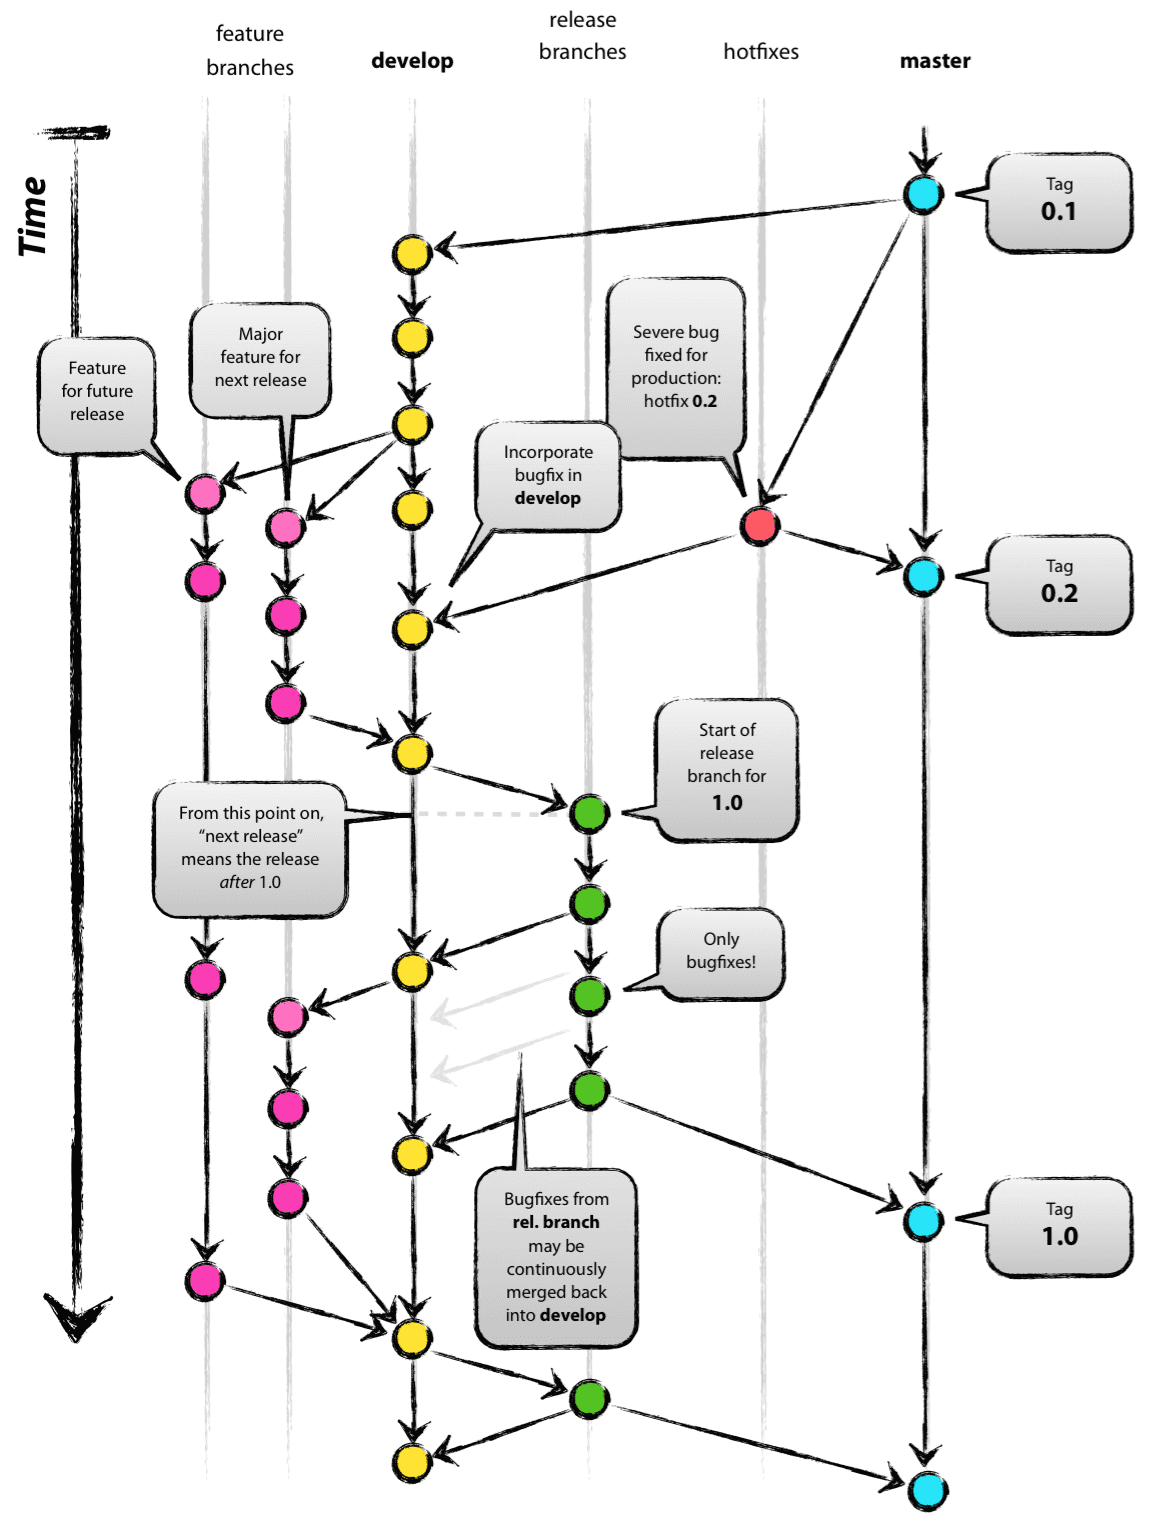
\includegraphics[width=0.6\linewidth]{config-management/gitflow}
\end{center}
% https://www.atlassian.com/git/tutorials/comparing-workflows/gitflow-workflow
%
% git branch develop
% git push -u origin develop
%
% git checkout -b develop origin/develop
% git checkout -b feature/jgitflow develop
% ..
% git commit -m
% git pull origin develop
% git checkout develop
% git merge feature/jgitflow
% git push
% git branch -d feature/jgitflow
\newslide
%\section{Github, Gitlab, Bitbucket}

\subsection{Software und weitere Informationen}
\begin{itemize}
\item Git Projekt-Seite: \href{http://git-scm.com/}{git-scm.com}
\item Git Tutorials: \href{http://www.gitguys.com}{www.gitguys.com},
   \href{https://www.atlassian.com/git/tutorials}{www.atlassian.com/git/tutorials}
\item 8 ways to share your git repository (Patrick Debois):\\
  \href{http://agile.dzone.com/news/8-ways-share-your-git}
   {}http://agile.dzone.com/news/8-ways-share-your-git
\item Git Workflows \href{https://www.atlassian.com/git/workflows}
         {www.atlassian.com/git/workflows}
\item Pro Git (Benutzeranleitung)
  \href{http://progit.org/book}{progit.org/book}
\item Git Reference: \href{http://gitref.org}{gitref.org}
\item Git -- Verteilte Versionsverwaltung für Code und Dokumente,
(V. Haenel, J. Plenz, Open Source Press, 2011)
\href{http://gitbu.ch}{gitbu.ch}
\item Eclipse-Plugin EGit:
  \href{http://www.eclipse.org/egit}{www.eclipse.org/egit}
\item TortoiseGit: \href{http://code.google.com/p/tortoisegit}
    {code.google.com/p/tortoisegit}
\end{itemize}
%
%http://www.kernel.org/pub/software/scm/git/docs/everyday.html
%
% self signed certs:
%% get certificate
% openssl s_client -connect host:port -key our_private_key.pem -showcerts -cert our_server-signed_cert.pem
%
% save it in /etc/ssl/certs
%
%% clone:
% GIT_SSL_CAINFO=/etc/ssl/certs/rorcz_root_cert.pem \
%    git clone https://repo.or.cz/org-mode.git
%
%# Ensure all future interactions with origin remote also work
% cd org-mode
% git config http.sslCAInfo /etc/ssl/certs/rorcz_root_cert.pem

%
\newslide
\section{Exercise}
\begin{enumerate}
\item Perform the following steps on the data loader component:
\begin{itemize}
\item Create a repository (e.g. Github, Gitlab)
\item Push your code into that repository
\item Think about the following questions:\\
Which parts of the project should be in the repository?
Which parts of the project should NOT be in the repository?
\item Create a tag which marks the software with \verb|V0_1|
\item Verify in the web console (Github, Gitlab) if
everything is correct.
\item Create a branch a perform a modification on that branch.
\item Merge the branch into the master branch.
\end{itemize}

\end{enumerate}
%{\bfseries Bewertung:} Vollständigkeit, Korrektheit, Nachvollziehbarkeit
%, Anschaulichkeit
% patch -p0 -i ~/milestone2.patch
% patch -p0 -i ~/milestone3.patch
\newslide
\section{Software and further Informations}
\begin{itemize}
\item Konfigurationsmanagement mit Subversion,
  Ant und Maven (Gunther Popp) dpunkt.verlag, 2008
\label{lit:popp}
%\item CVS
%\begin{itemize}
%\item Die offizielle CVS-Projektseite:
%  \href{http://savannah.nongnu.org/projects/cvs/}
%    {savannah.nongnu.org/projects/cvs/}
%\item Open Source Development with CVS:
%  \href{http://cvsbook.red-bean.com}{cvsbook.red-bean.com}
%\item CVS Client/Server für Windows 2000/XP:
%  \href{http://www.march-hare.com/cvspro}{www.march-hare.com/cvspro}
%\item Ein CVS-Client-Front-End für MS-Explorer:
%  \href{http://www.tortoisecvs.org}{www.tortoisecvs.org}
%\item Mehrere graphische Frontends für CVS:
%  \href{http://www.wincvs.org}{www.wincvs.org}
%\end{itemize}
\item Weitere Versionsverwaltungs-Tools:
\begin{itemize}
\item Mercurial: \href{http://mercurial.selenic.com/}{mercurial.selenic.com}
\item Monotone:
  \href{http://www.monotone.ca}{www.monotone.ca}
\item GNU arch:
  \href{http://www.gnu.org/s/gnu-arch}{www.gnu.org/s/gnu-arch}
\end{itemize}
\end{itemize}
%---------------------------------------------------------------

%%% Local Variables:
%%% mode: latex
%%% TeX-master: t
%%% End:
